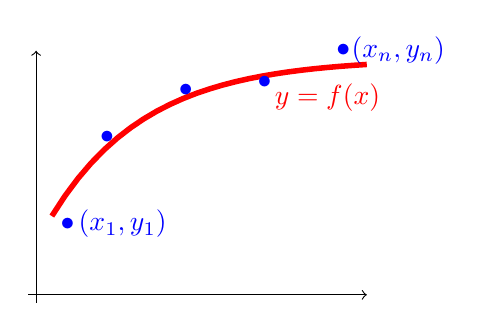
\begin{tikzpicture}[
    declare function={%
        F(\x)               =3-2*pow(2.7979,-0.8*\x); 
    }
 ]
    
    
    % Zeichnen der Funktion   
    \draw[red,line width=2pt,domain=0:4] plot({\x},{F(\x)});
    
    % Bezeichnung
    \node[red] (O) at(3.5,2.5) {$y=f(x)$};
    
    % Punkte
    \node[blue] (P1n) at (0.9,0.9) {$(x_1,y_1)$};
    \node[blue] (P1) at (0.2,0.9) {$\bullet$};
    
   \node[blue] (P2) at (2.7,2.7) {$\bullet$};
   \node[blue] (P3) at (1.7,2.6) {$\bullet$};
   \node[blue] (P4) at (0.7,2) {$\bullet$};
   
   \node[blue] (P5n) at (4.4,3.1) {$(x_n,y_n)$};
   \node[blue] (P5) at (3.7,3.1) {$\bullet$};
   
   % Koordinatensystem
   \draw[color=black,->] (-0.2,-0.1) -- (-0.2,3.1); 
   \draw[color=black,->] (-0.3,0) -- (4,0); 
\end{tikzpicture}
